\section{Horizontal gedrehtes 3-Schicht-System}
\subsection{Betrachtung des gedrehten Probendesigns}
In diesem Abschnitt soll das im vorherigen Kapitel beschriebene 3-Schicht-System (\cref{fig:cu_unter_fe}) horizontal im mathematisch negativen Sinne um \SI{45}{\degree} gedreht werden, was ein Wiederverwenden der alten Probe und eine Überprüfung der Simulation auf Konsistenz außerhalb der Symmetrieachsen ermöglicht. Dies ist nachfolgend in \cref{fig:45grad} dargestellt.

\begin{figure}[H] 
  \centering
     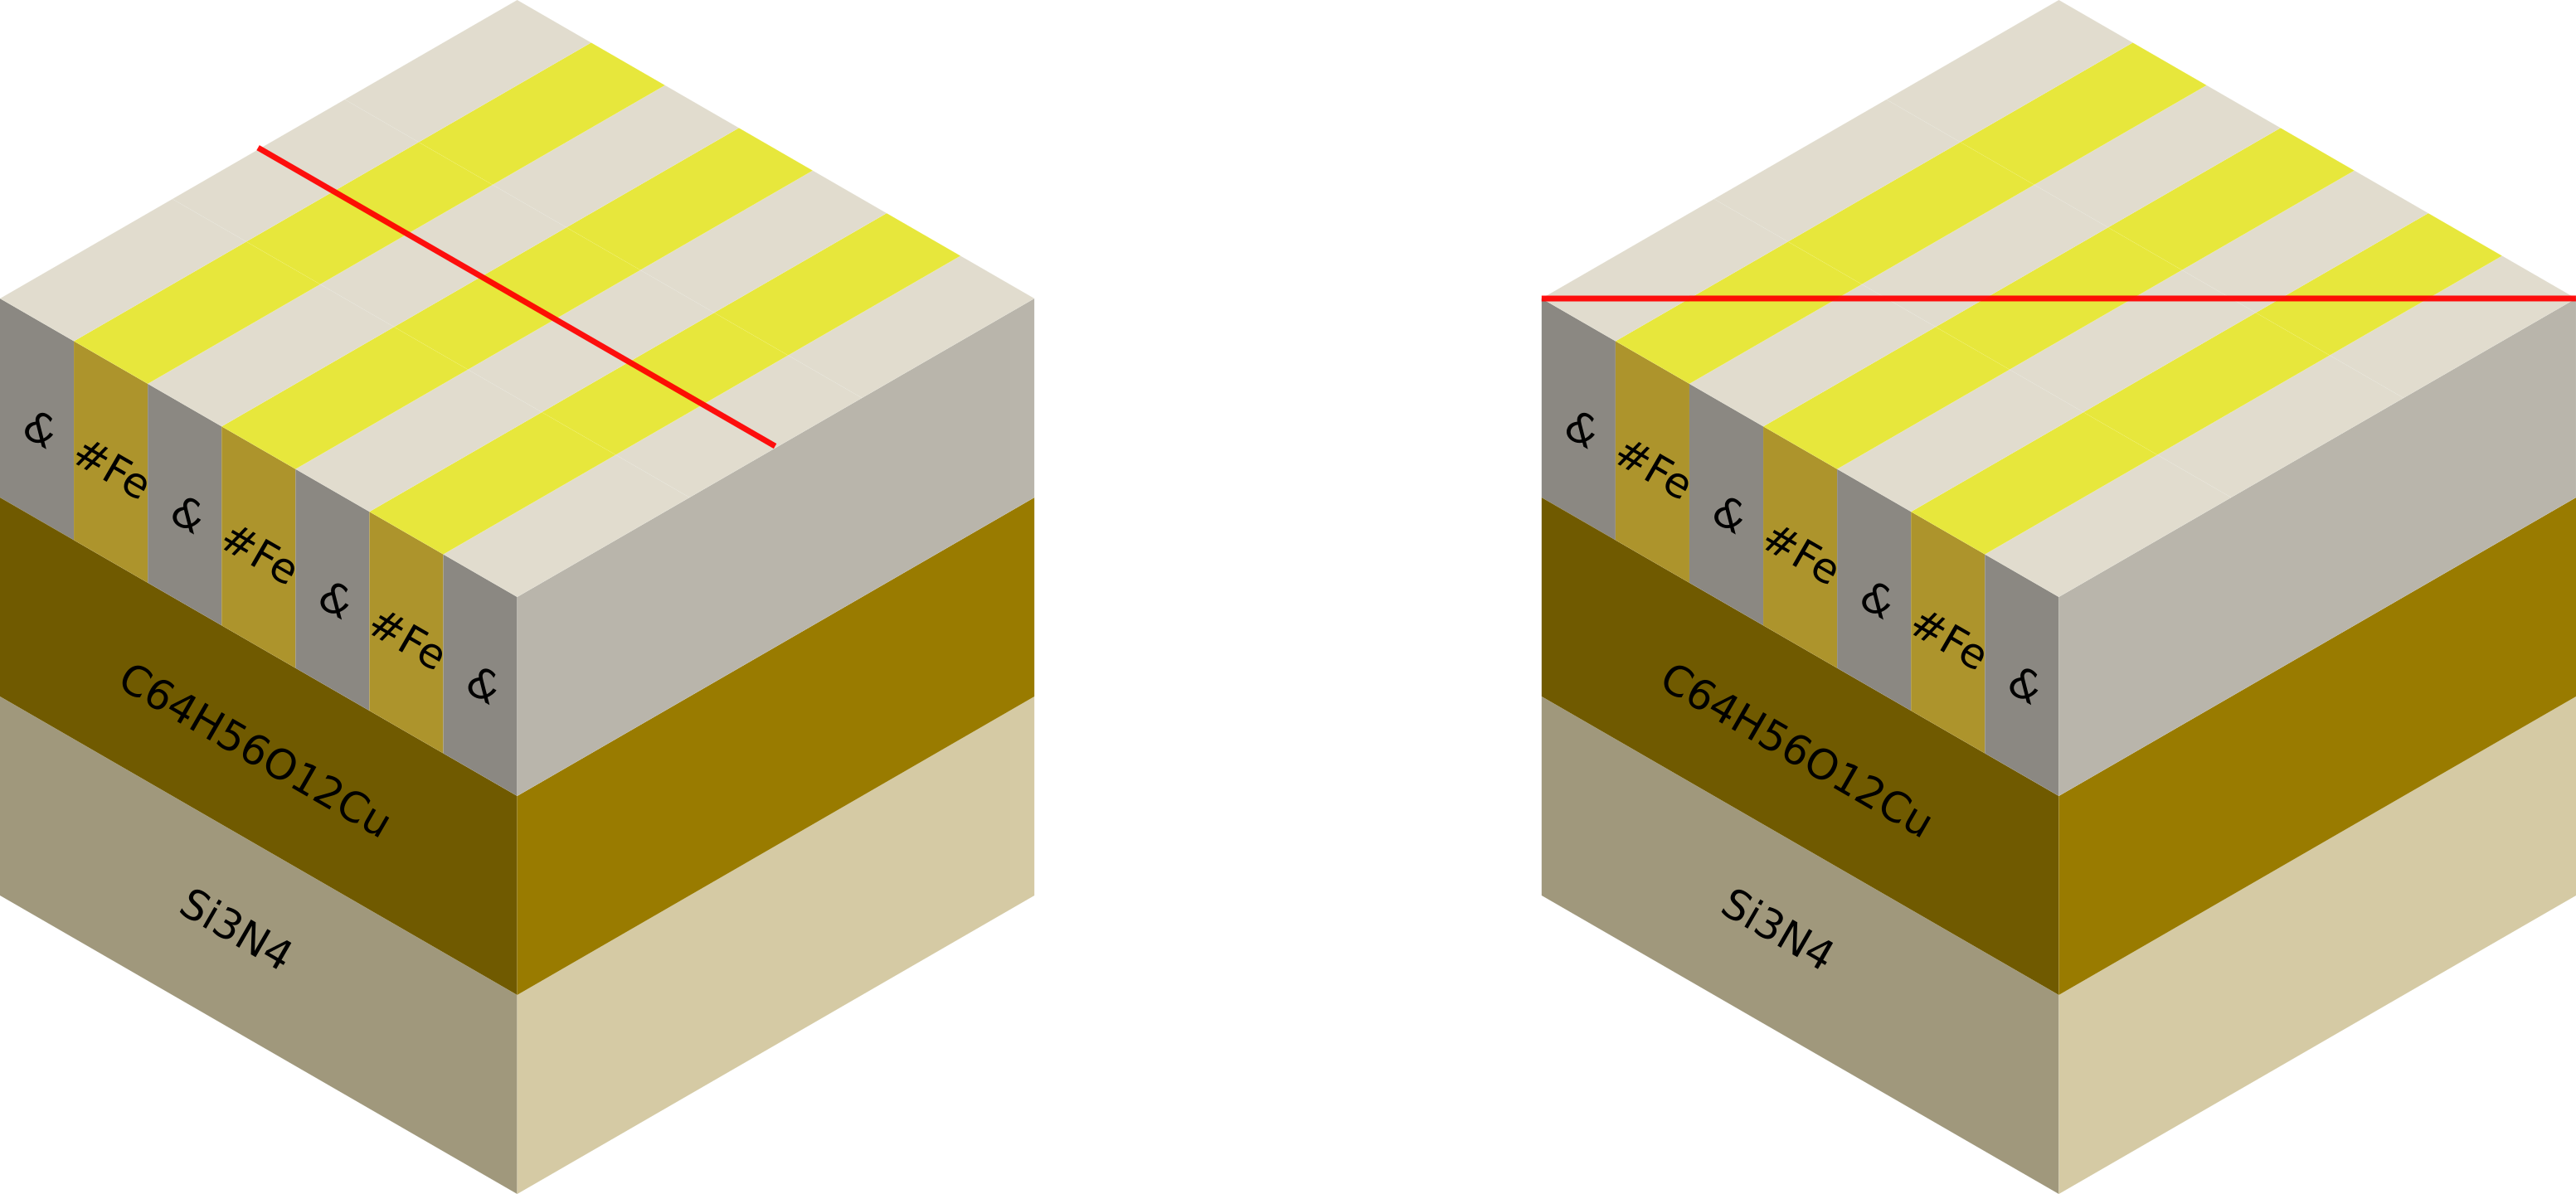
\includegraphics[width=0.85\textwidth]{illustrations/45grad.png}
  \caption[Gedrehtes 3-Schicht-System]{Illustriert ist die veränderte Scanrichtung bei Drehung des 3-Schicht-Systems um \SI{45}{\degree} (rechts). Wie vorher befindet sich auf einem Siliziumnitridfenster eine Ebene, welche aus einem Lack mit zugemischtem Kupfer besteht. Die darüberliegende Ebene ist ein Schichtwechsel einer Speziallackschicht ohne Eisenanteil ($\&$) und des Lacks mit beigemischtem Eisenanteil ($\#Fe$). Aus darstellungstechnischen Gründen ist die Scanrichtung, nicht die Probe gedreht.}
  \label{fig:45grad}
\end{figure}


Bei Beibehalten der Scanrichtung ändert sich durch die Drehung die detektierte Probengeometrie für die 4 Detektoren grundlegend. So ist nun nicht mehr davon auszugehen, dass je zwei nebeneinanderliegende Detektorsegmente das gleiche Signal erkennen, sondern der Absorptionspfad vor einer Fe-Schicht wird für einen Detektor maximiert, für den Anderen minimiert und für 2 diagonal gegenüberliegende Detektoren sollten die selben Daten simuliert werden.

\begin{figure}[H] 
  \centering
     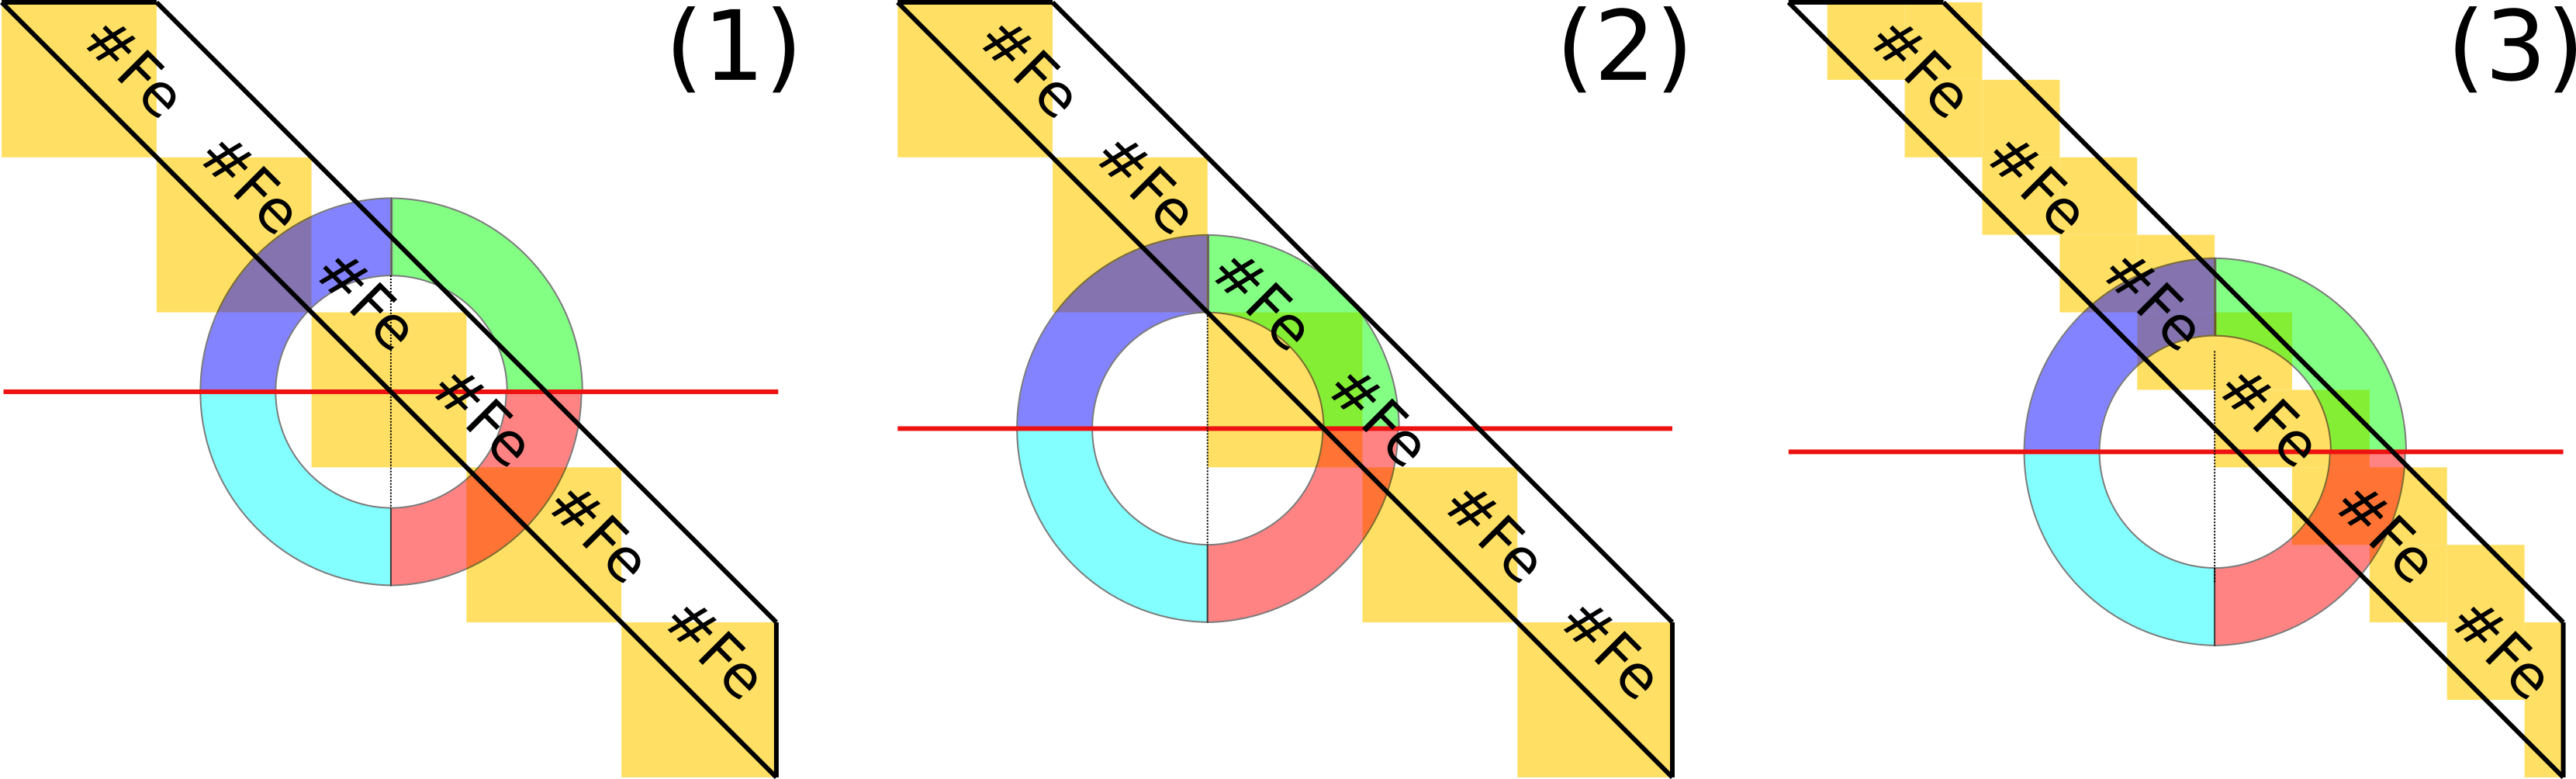
\includegraphics[width=0.85\textwidth]{illustrations/45grad_challenge.png}
  \caption[Gegenüberstellung: großes und kleines Raster]{Simplifizierte oberste Ebene der Probe. Der Detektor ist als bunte Ringscheibensegmente (blau[1], grün[2], rot[3], türkis[4]), die Scanrichtung ist in rot abgebildet. Außerdem eine Eisenschicht der Probe im \SI{45}{\degree} Winkel (schwarz umrandet, beschriftet) und die gerasterte Umsetzung in der QUADaps Software (gelb). Fall (1): Rasterpunkt liegt zentral im Quadrat; symmetrisches Signal für Detektor 1+3. Fall (2): Anregung unterhalb der zentralen Achse an Probenoberfläche; die von Detektor 3 berechnete Fluoreszenzstrahlung erfährt deutlich weniger Absorption durch die Eisenschicht. Fall (3): wie Fall (2), jedoch deutlich feineres Raster; Signale für Detektor 1+3 immernoch unterschiedlich, jedoch deutlich ähnlicher.}
  \label{fig:45grad_challenge}
\end{figure} 

Die Drehung der Probe um \SI{45}{\degree} gegenüber dem Detektor (\cref{fig:45grad}) stellt die QUADaps Software vor eine Herausforderung, da diese für Proben, welche Eckig sind und deren Kanten senkrecht oder parallel zur Scanrichtung liegen, konzipiert wurde. Dadurch können Proben, welche diese Bedingungen nicht erfüllen, wie beispielsweise eine runde Struktur oder, wie in diesem Fall, eine Struktur, die um \SI{45}{\degree} gedreht wurde, nur sehr schwer dargestellt werden. Genauer muss die Struktur durch ein Raster approximiert werden. Ist eine genauere Approximation gewünscht müssen die Segmente kleiner angelegt werden und die Menge an Rasterelementen steigt an. Soll die Struktur in x- sowie in y-Richtung doppelt so fein abgebildet werden, so besitzt das dazugehörige Raster 4 mal so viele Elemente. Beispielhaft ist eine solche Approximation in \cref{fig:45grad_challenge} dargestellt. Eine schräge Struktur wird durch Quadrate approximiert. Die Genauigkeit der Simulationsergebnisse hängt maßgeblich von der Feinheit des Rasters ab, da durch ein feineres Raster andere neue Effekte korrigiert werden können. Beispielsweise sollte darauf geachtet werden, dass mittig an einem der Quadrate gemessen wird, da sonst schräg gegenüberliegende Detektoren unterschiedliche Signale liefern. Dies ist als Draufsicht in \cref{fig:45grad_challenge} (2) dargestellt. Die Austrittswinkel $\alpha$ und $\beta$ wurden zu einer Ringscheibe zusammengefasst, ein Quadrant ist je einem Detektor zugeordnet. In (2) wird die von Detektor 4 (blau) detektierte Strahlung deutlich mehr durch eine Fe-Lackschicht abgeschwächt, als die von Detektor 2 (rot) obwohl die reale Struktur symmetrisch gegenüber dieser Achse ist. Zum Vergleich findet sich unter (3) ein doppelt so feines Raster bei dem sich die durch Eisen transmittierten Flächen weiter angleichen. 



\subsection{Simulation}
Bei einer ursprünglichen Schichtbreite von \SI{3.7}{\micro\meter} ergibt sich die Breite der um \SI{45}{\degree} gedrehten Probe zu $\sqrt{2 \cdot \SI{3.7}{\micro\meter} \cdot \SI{3.7}{\micro\meter}} = \SI{5.2}{\micro\meter}$. Die Feinheit des Abrasterns der Probe wird auf \SI{50}{\nano\meter} pro Schritt gesetzt, die übrigen Parameter wurden beibehalten. Die Kantenlänge des Probenraster wurde zu \SI{0.4}{\micro\meter} gewählt. Dadurch ergibt sich eine Matrix mit etwa 10.000 Einträgen. Verglichen mit dem ungedrehten 3-Schicht-System ist diese Matrix etwa 1.000-mal größer. Dies zeigt wie aufwändig der Entwurf von inhomogenen Proben bzw. Proben, welche nicht eckig und symmetrisch bezüglich des internen Koordinatensystems sind, ist. Die Resultate der etwa 19-stündigen Simulation sind nachfolgend abgebildet.

\begin{figure}[H] 
  \centering
     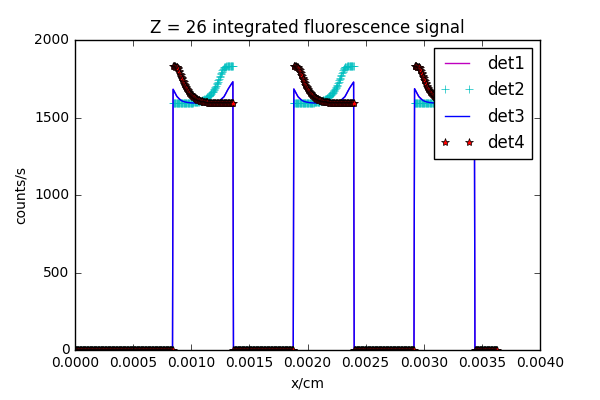
\includegraphics[width=0.85\textwidth]{illustrations/45grad_fe.png}
  \caption[Fluoreszenzbild Eisen \SI{45}{\degree}-Probe]{Dargestellt ist das Fluoreszenzsignal von Eisen in dem um \SI{45}{\degree} gedrehten 3-Schicht-System welches über Quadrate mit einer Kantenlänge von \SI{0.4}{\micro\meter} approximiert wurde. Die Kurvenverläufe sind durch Selbstabsorptionseffekte bedingt.}
  \label{fig:45grad_fe}
\end{figure}

Das detektierte Fe-Fluoreszenzsignal ist in \cref{fig:45grad_fe} abgebildet. Für die Detektoren 2+4 gelten die Betrachtungen der Selbstabsorptionseffekte analog zu \cref{fig:cu_fe_fe_signal} jedoch ist an den Schichtgrenzen ein kurzes Plateau zu erkennen. Die detektierten Fluoreszenzlinien der Detektoren 1+3 liegen übereinander. Anhand der unterschiedlichen Peakhöhen an den Schichtgrenzen ist bereits hier mit bloßem Auge zu erkennen, dass die Feinheit des Rasters für sehr präzise Ergebnisse nicht ausreichend ist, da es sich um eine symmetrische Geometrie handelt und somit die Peaks die gleiche Höhe besitzen sollten.

\begin{figure}[H] 
  \centering
     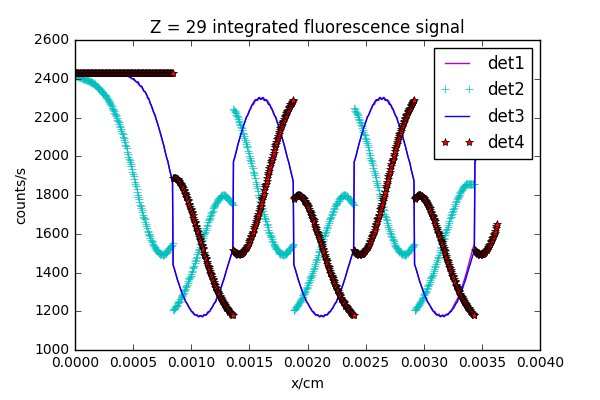
\includegraphics[width=0.85\textwidth]{illustrations/45grad_cu.png}
  \caption[Fluoreszenzbild Kupfer \SI{45}{\degree}-Probe]{Die Kurvenverläufe zeigen das detektierte Cu-Fluoreszenzsignal des gedrehten 3-Schicht-Systems. Die Signale der Detektoren 1+3 sind identisch. Legt man das eine vertikale Gerade durch das Maximum bei $x\approx$\SI{17}{\micro\meter} sieht man, dass das Fluoreszenzbild um diese Vertikale auf beiden Seiten nicht ganz symmetrisch ist, wie bereits in \cref{fig:45grad_fe}. Außerdem sind für alle Detektoren Sprünge an den Schichtgrenzen durch die Abschwächung der Anregungsintensität in den Fe-Schichten zu erkennen, sowie das Abfallen und Ansteigen durch die Absorption in der darüber liegenden alternierenden Schicht.}
  \label{fig:45grad_cu}
\end{figure}

Nachfolgend werden anhand von \cref{fig:45grad_cu} die Verläufe der Kurven der Cu-Fluoreszenz\-signale beginnend an der ersten Schichtgrenze bei $x\approx$ \SI{8}{\micro\meter} diskutiert. Der Verlauf der übereinander liegenden Fluoreszenzsignale der Detektoren 1+3 lässt sich durch Absorptionseffekte beschreiben. So fällt in der Nähe vor der ersten Fe-Schicht das Signal langsam ab, da bereits hier ein Teil der Fluoreszenzstrahlung von den Fe-Partikeln absorbiert wird. Zur Veranschaulichung bewege man gedanklich den Detektor in \cref{fig:45grad_challenge} (2) etwas nach links. Auf den kontinuierlichen Abfall folgt an der Schichtgrenze ein Sprung. Dieser lässt sich dadurch erklären, dass die Anregungsintensität bereits vor der Fluoreszenzanregung durch die Fe-Schicht abgeschwächt wird. Dies ist auch in \cref{fig:cu_fe_cu_signal} zu Beobachten. Der Absorptionsweg durch die Fe-Schicht wird immer länger, die detektierten Counts fallen weiter ab. Mittig in der Fe-Schicht ist das Minimum der detektierten Fluoreszenzintensität, daraufhin wird der Absorptionsweg durch die Fe-Schicht wieder kürzer, demzufolge steigt die Intensität. Die nachfolgende Sprungstelle ist analog zu der Vorherigen zu erklären, jedoch steigt nun die Intensität wieder, da durch die leichte Lackschicht transmittiert wird. Bemerkenswert ist, dass die Fluoreszenzkurve gegenüber seinem Minimum bzw. Maximum nicht perfekt symmetrisch ist. Dies muss an der Approximation der schrägen Struktur durch Quadrate liegen (vergleiche \cref{fig:45grad_challenge}).\newline

Ausgehend von der Schichtgrenze bei $x\approx$ \SI{8}{\micro\meter} nimmt das von Detektor 2 gemessene Fluoreszenzsignal stetig zu, da sich dieser (in Scanrichtung betrachtet) hinter der Fe-Schicht befindet. Daher wird im weiteren Verlauf der Absorptionsweg durch die Fe-Schicht immer kürzer, bis er kurz vor dem Schichtwechsel sein Minimum erreicht. Im Fluoreszenzsignal ist dies jedoch nur ein lokales Maximum, da der Sprung an der Schichtgrenze groß ist. Dieses Phänomen des lokalen Maximums innerhalb der Fe-Schicht vor der Schichtgrenze und analog des lokalen Minimums in der leichten Schicht konnten in den bisherigen Proben nicht beobachtet werden. Vermutlich liegt dies daran, dass Fluoreszenz, welche tief in der Cu-Lackschicht emittiert wird genau dann maximal absorbiert wird, wenn der Absorptionsweg durch die Fe-Lackschicht maximal ist. Dies liegt für tiefere Emission ein Stück vor der Schichtgrenze, zur Visualisierung dieses Effekts kann der Anregungspunkt in \cref{fig:strahlengang} entlang $c_a$ ein Stück in die Siliziumschicht bewegt werden. Warum dieser Effekt jedoch vorher nicht beobachtet wurde, ist unklar und bedarf weiterer Untersuchung.\newline
Die Betrachtung für Detektor 4 verläuft analog. Einzige Unterschiede sind einerseits keine perfekte Spiegelsymmetrie zu Detektor 2, dies ist aber vermutlich erneut durch die Approximation des schrägen Designs bedingt. Außerdem ist aufgrund des Beobachtungsorts und der Definition der Ränder der Bereich vor der ersten Schichtgrenze konstant und die in der ersten Eisenschicht gemessenen Intensitäten etwas höher.\newline

Aufgrund des neuen Phänomens ist zusammenfassend zu sagen, dass auf eine Untersuchung einer bereits bekannten Probe unter gedrehtem Winkel nicht verzichtet werden sollte. Außerdem sollte eine weitere vergleichende Simulation mit noch feiner approximierten Probenstrukturen sowie deutlich kleineren Schrittweiten für die Scans angelegt werden.